%%
%% $Id$
%%
%% Copyright 1989-2014 MINES ParisTech
%%
%% This file is part of PIPS.
%%
%% PIPS is free software: you can redistribute it and/or modify it
%% under the terms of the GNU General Public License as published by
%% the Free Software Foundation, either version 3 of the License, or
%% any later version.
%%
%% PIPS is distributed in the hope that it will be useful, but WITHOUT ANY
%% WARRANTY; without even the implied warranty of MERCHANTABILITY or
%% FITNESS FOR A PARTICULAR PURPOSE.
%%
%% See the GNU General Public License for more details.
%%
%% You should have received a copy of the GNU General Public License
%% along with PIPS.  If not, see <http://www.gnu.org/licenses/>.
%%

%% Documentation for XPOMP

\documentclass[a4paper]{article}
\usepackage{epsfig,xspace,hyperref,verbatim}
%%\usepackage{page_de_garde_CRI}
\begin{document}
\newcommand{\CRI}{\htmladdnormallink{Centre de Recherche en Informatique}
  {http://www.cri.ensmp.fr}\xspace}
\newcommand{\HPFC}{\htmladdnormallink{\texttt{HPFC}}
  {http://www.cri.ensmp.fr/pips/hpfc.html}\xspace}
\newcommand{\xPOMP}{\htmladdnormallink{\textbf{xPOMP}}
  {http://www.cri.ensmp.fr/pips/xpomp_manual/xpomp_manual.html}\xspace}
\newcommand{\POMP}{\htmladdnormallink{\textbf{POMP}}
  {ftp://ftp.ens.fr/pub/pomp}\xspace}
\newcommand{\POMPC}{\htmladdnormallink{\textbf{POMPC}}
  {ftp://ftp.ens.fr/pub/pompc}\xspace}
\newcommand{\HyperC}{\textbf{HyperC}\xspace}
\newcommand{\PIPS}{\htmladdnormallink{\textbf{Pips}}
  {http://www.cri.ensmp.fr/pips}\xspace}
\newcommand{\FC}{\htmladdnormallink{Fabien \textsc{Coelho}}
  {http://www.cri.ensmp.fr/people/coelho}\xspace}
\newcommand{\Xonze}{\htmladdnormallink{\textbf{X11}}
  {http://www.x.org}\xspace}

%% Stack up all the figures and the text:
\renewcommand{\floatpagefraction}{1}
\renewcommand{\textfraction}{0}
\renewcommand{\topfraction}{1}
\renewcommand{\bottomfraction}{1}

\date{1996/12/20}

\newcommand{\numerocri}{A/298-CRI}
\newcommand{\titre}{xPOMP\\
  a Simple X11 graphical Library to Display Arrays in C,
  Fortran and HPF}
\newcommand{\auteur}{Ronan \textsc{Keryell}\\
  Nicolas \textsc{Paris}}
\newcommand{\docdate}{\today}
\newcommand{\lieu}{}
%%\SortLaPageDeGarde


\title{xPOMP: a Simple X11 graphical Library to Display Arrays in C,
  Fortran and HPF\\
  ---\\
  Technical Report A/CRI/298}
\author{Ronan \textsc{Keryell}\thanks{%
    \CRI,
    \htmladdnormallink{�cole Nationale Sup�rieure des Mines de Paris}
    {http://www.ensmp.fr},
    35, rue Saint-Honor�,
    F-77305 \textsc{Fontainebleau cedex, France},
    \texttt{\htmladdnormallink{keryell@cri.ensmp.fr}
      {mailto:keryell@cri.ensmp.fr}}.}
  \and Nicolas \textsc{Paris}\thanks{%
    \htmladdnormallink{\textsc{ais} Berger-Levrault}
    {http://www.Berger-Levrault.fr},
    34, Avenue du Roul�, F-92200 \textsc{Neuilly sur Seine, France},
    \texttt{\htmladdnormallink{nico@Berger-Levrault.fr}
      {mailto:nico@Berger-Levrault.fr}}.}
  }

\maketitle

\begin{abstract}
  \xPOMP is a small graphical interface able to open X11 windows and
  display user bidimensional array values as images with a mapping
  between element value and pixel color. The programming interface is
  quite simple and is available for the C, Fortran and HPF languages.
\end{abstract}

\begin{quotation}
  \centerline{\textbf{R�sum�}}
  \emph{\small%
    \xPOMP est une petite interface graphique capable d'ouvrir
    plusieurs fen�tres X11 pour afficher des tableaux bidimensionnels
    sous forme d'images dont la couleur des pixels d�pend de la valeur
    des �l�ments de tableau. L'interface de programmation est
    tr�s simple et est disponible pour les langages C, Fortran et HPF.%
    }
\end{quotation}

\section{Introduction}
\label{sec:introduction}

Visualization is a powerful tool to explore data but also to help
debugging programs, specially parallel programs where bugs are often
emphasized. \xPOMP is such a tool and can display 2-dimensionnal arrays
in XWindowS 11 windows as a part of the \PIPS project but it can be
used independently.

The interface is quite simple to let the user focusing on its
application but it provides some nice features like color map
selection, mouse interaction, frame drawing, etc. The interface is
available for C and Fortran languages, and also HPF since it it used
with the HPF compiler \HPFC at the \CRI in the \PIPS project.

The \xPOMP philosophy usage is to open as much as wanted X11 windows
with \verb|XPOMP_open_display()|. In each window, some arrays can be
mapped and displayed with one color map per window.

Resources can be freed later with \verb|XPOMP_close_display()| even if
the window itself is not unmapped (type \verb|q| to remove it).

Some fancy usage for debugging is to use \xPOMP to add graphical array
display features to a debugger. Just ask the debugger to
\verb|display| (for \texttt{dbx} or \texttt{gdb}) a call to
\verb|XPOMP_show_double()| of an array and \verb|XPOMP_scroll()|.

\xPOMP, like \HyperC from HyperParallel Technologies, is based on
previous work from the \POMP{}/\POMPC project at
\htmladdnormallink{�cole Normale Sup�rieure de
  Paris}{http://www.ens.fr}.



\section{User manual}
\label{sec:user}

From the user point of view, an \xPOMP window is a X11 window as shown
on Figure~\ref{fig:xPOMP_window}. It uses its own X11 colormap to
display a 256-level image.

\begin{figure}
  \begin{center}
    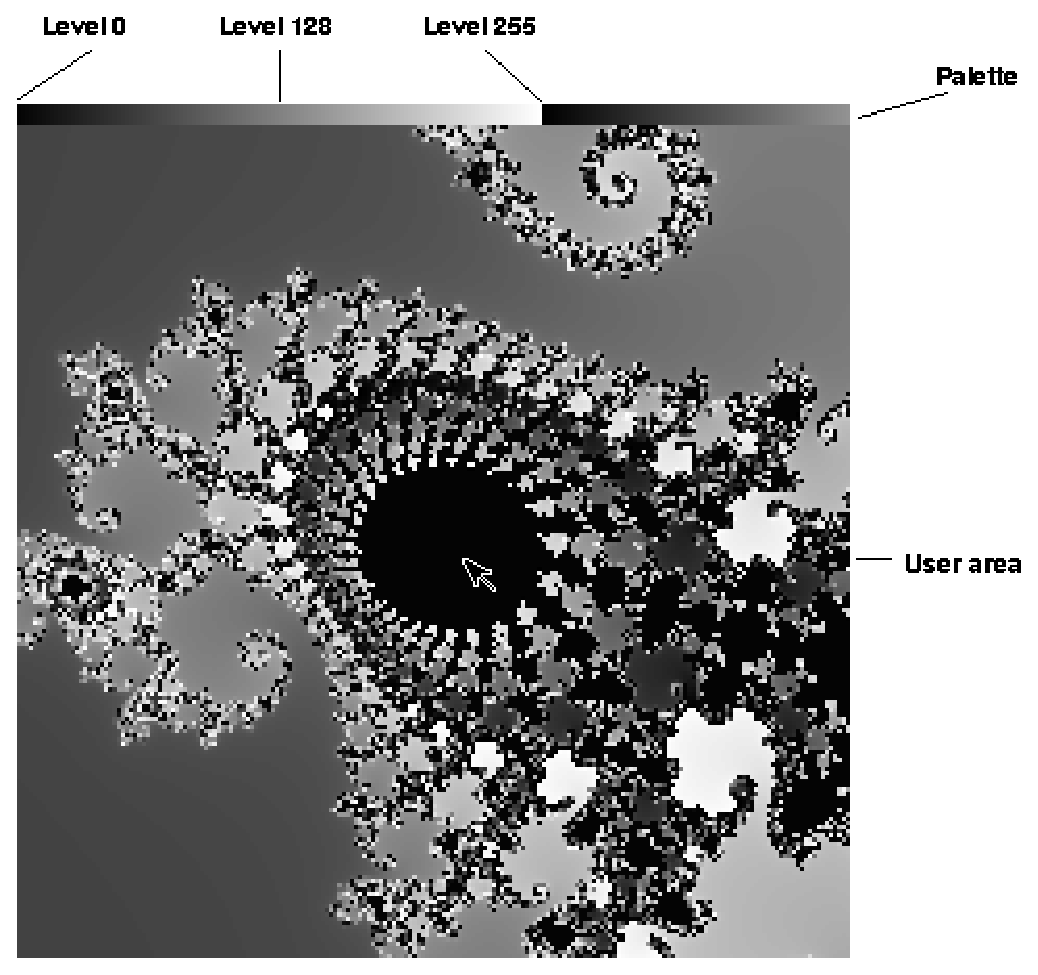
\psfig{file=xPOMP_window_explained,width=\hsize}    
  \end{center}
  \caption{Example of an \xPOMP window displaying a fractal.}
  \label{fig:xPOMP_window}
\end{figure}

Such a window is splitted in 2 parts:
\begin{itemize}
\item a color map area that displays the colors scale from level 0 to
  level 255 from left to right. If the window width is less than 256,
  not all the color map is displayed but if the width is greater than
  256, the same color map is concatenated to fill the width ;
\item a user area where some arrays can be displayed, with the origin
  at the top left corner of the user area.
\end{itemize}

The mouse buttons can be used to send events to the application
program and the actions, if any, are defined by this application
program.

Many keystrokes can be used to control the \xPOMP viewer:
\begin{description}
\item[q or \^{}D:] quit the viewer window;
\item[color map type selection] ~
  \begin{description}
  \item[1:] grey scale;
  \item[2:] rainbow color;
  \item[3:] rainbow color with alternating half-tone. Useful to
    display small level differences;
  \item[4:] color centered, from blue to red. This color map is not
    linear and is useful to separate a small level zone;
  \item[0:] use the application defined color map if any;
  \end{description}
\item[color map parameters] ~
  \begin{description}
  \item[- or \_:] decrease the cycling rate of the color map;
  \item[+ or =:] increase the cycling rate of the color map;
  \item[h]: increase start value;
  \item[l:] decrease start value;
  \item[j:] decrease clipping level value;
  \item[k:] increase clipping level value;
  \item[H:] combination of 'h' and 'j' keys;
  \item[L:] combination of 'k' and 'l' keys;
  \item[?:] print out the actual color map parameters.
  \end{description}
\end{description}

\section{Programmer manual}
\label{sec:programmer}

An application program can open one or more \xPOMP windows to display
various numerical information. Each window can contain several array
image and the application program can get user feed back from the
mouse.

Each library function or procedure has 2 different definition
templates, one for the C language and another one for the Fortran
language. C function or procedure names begin with \verb|XPOMP_| but
Fortran ones begin with \verb|xpompf|.

To declare the interface functions or procedures, one must include the
\xPOMP header file with
\begin{verbatim}
#include <xpomp_graphic.h>
\end{verbatim}
in C or
\begin{verbatim}
      include 'xpomp_graphic_F.h'
\end{verbatim}
in Fortran.



\subsection{Window manipulation}

\subsubsection{Opening a new window}

The first thing to do is to open a new \xPOMP window by calling the
function\\
C:
\begin{verbatim}
XPOMP_display window;
int X_window_size, Y_window_size;
window = XPOMP_open_display(X_window_size, Y_window_size);
\end{verbatim}
Fortran:
\begin{verbatim}
       integer window
       integer X_window_size, Y_window_size
       call xpompf open_display(X_window_size, Y_window_size, window)
\end{verbatim}

This function open a window with a user area of pixel size
\verb|X_window_size|$\times$\verb|X_window_size| and return a window
handler in \verb|window|.

The background color is set to color 1.


\subsubsection{Closing a window}

The following procedures close the window connection
\verb|window|. Note that the \xPOMP window itself is not unmapped and
remain displayed.\\
C:
\begin{verbatim}
XPOMP_display window;
XPOMP_close_display(window);
\end{verbatim}
Fortran:
\begin{verbatim}
       integer window
       call xpompf close display(window)
\end{verbatim}



\subsection{Selecting a default display}

Most of \xPOMP routines can accept a display by default by giving them
the $-1$ handler value. If none default display exist, a new window is
created and it becomes the default window.

But the user can select a window as the default one by calling the
following functions that return the handler of the previous default
display if any or $-1$.\\
C:
\begin{verbatim}
XPOMP_display new_default_window, old_default_window;
old_default_window = XPOMP_set_current_default_display(new_default_window);
\end{verbatim}
Fortran:
\begin{verbatim}
       integer new_default_window, old_default_window
       call xpompf set current default display
      &    (new_default_window,old_default_window)
\end{verbatim}


\subsubsection{Getting the default window handler}

The default window handler (if any or $-1$) is returned by the following
functions:\\
C:
\begin{verbatim}
XPOMP_display default_window;
default_window = XPOMP_get_current_default_display();
\end{verbatim}
Fortran:
\begin{verbatim}
       integer default_window
       call xpompf get current default display(default_window)
\end{verbatim}


\subsubsection{Getting the display depth}

Since it may be useful to know the bit size of the window ixel to
display informations accordingly, this size is returned by:\\
C:
\begin{verbatim}
int depth;
default_window = XPOMP_get_depth();
\end{verbatim}
Fortran:
\begin{verbatim}
       integer depth
       call xpompf get depth(depth)
\end{verbatim}

On failure, the value $-1$ is returned instead of the depth.


\subsection{Displaying data}

\xPOMP can display array information in two way, one with character
type to directly control color or one with floating point type that is
mapped on the color color map.


\subsubsection{Displaying a character array}
\label{sec:xpomp_flash}

The following functions display an unsigned character vector
considered as an array of size
\texttt{X\_data\_array\_size}$\times$\texttt{Y\_data\_array\_size} at
position $(\texttt{X\_offset},\texttt{Y\_offset})$ on the window
\texttt{window}. Each pixel will have a size
\texttt{X\_zoom\_ratio}$\times$\texttt{Y\_zoom\_ratio}.  The functions
return 0 on success, $-1$ on failure. Each character value directly
control the color pixel through the color color map: value 0 will be
displayed with color map color 0 up to value 255 displayed with color
map color 255. It is thus considered as an uncooked
mode.\\
C:
\begin{verbatim}
unsigned char * data_array;
int X_data_array_size, Y_data_array_size;
int X_offset, Y_offset;
int X_zoom_ratio, Y_zoom_ratio;
int status;
status = XPOMP_flash(window,
                     data_array,
                     X_data_array_size, Y_data_array_size,
                     X_offset, Y_offset,
                     X_zoom_ratio, Y_zoom_ratio);
\end{verbatim}
Fortran:
\begin{verbatim}
      integer window
      integer X_data_array_size, Y_data_array_size
      character image(0:X_data_array_size - 1, 0:Y_data_array_size - 1)
      integer X_offset, Y_offset
      integer X_zoom_ratio, Y_zoom_ratio
      integer status
      call xpompf flash(window, data_array,
     &                 X_data_array_size, Y_data_array_size,
     &                 X_offset, Y_offset,
     &                 X_zoom_ratio, Y_zoom_ratio, status)
\end{verbatim}


\subsubsection{Displaying a floating point array}

\xPOMP allows the representation of floating point array whose values
are mapped to color map color 1 to 254 (and not 0 to 255 to spare some
colors to be displayed as a clip layer or to detect overload). The
user given values \verb|min_value| and \verb|max_value| fix the value
matching color 1 and color 254. If the given values are both 0, these
values are set internally to the minimum and maximum values of array
elements.

Other parameters are the same as for Section~\ref{sec:xpomp_flash}.

Functions return $0$ when successful, $-1$ otherwise.

Since floating point value are often stored as single or double
precision that does not use the same memory storage, two different
interfaces exist.


\paragraph{Single precision interface}

\noindent
C:
\begin{verbatim}
XPOMP_display window;
float * image;
int X_data_array_size, Y_data_array_size;
int X_offset, Y_offset;
int X_zoom_ratio, Y_zoom_ratio;
double min_value, max_value;
int status;
status = XPOMP_show_float(screen, image,
                          X_data_array_size, Y_data_array_size,
                          X_offset, Y_offset,
                          X_zoom_ratio, Y_zoom_ratio,
                          min_value, max_value);
\end{verbatim}
Fortran:
\begin{verbatim}
      integer window
      integer X_data_array_size, Y_data_array_size
      real*4 image(0:X_data_array_size - 1, 0:Y_data_array_size - 1)
      integer X_offset, Y_offset
      integer X_zoom_ratio, Y_zoom_ratio
      integer status
      real*8 min_value, max_value;
      integer status
      call xpompf show real4(screen, image,
     &                      X_data_array_size, Y_data_array_size,
     &                      X_offset, Y_offset,
     &                      X_zoom_ratio, Y_zoom_ratio,
     &                      min_value, max_value, status)
\end{verbatim}


\paragraph{Double precision interface}

\noindent
C:
\begin{verbatim}
XPOMP_display window;
double * image;
int X_data_array_size, Y_data_array_size;
int X_offset, Y_offset;
int X_zoom_ratio, Y_zoom_ratio;
double min_value, max_value;
int status;
status = XPOMP_show_double(screen, image,
                           X_data_array_size, Y_data_array_size,
                           X_offset, Y_offset,
                           X_zoom_ratio, Y_zoom_ratio,
                           min_value, max_value);
\end{verbatim}
Fortran:
\begin{verbatim}
      integer window
      integer X_data_array_size, Y_data_array_size
      real*8 image(0:X_data_array_size - 1, 0:Y_data_array_size - 1)
      integer X_offset, Y_offset
      integer X_zoom_ratio, Y_zoom_ratio
      integer status
      real*8 min_value, max_value
      integer status
      call xpompf show real8(screen, image,
     &                      X_data_array_size, Y_data_array_size,
     &                      X_offset, Y_offset,
     &                      X_zoom_ratio, Y_zoom_ratio,
     &                      min_value, max_value, status)
\end{verbatim}


\subsection{Color Map operation}

Several type of color map exists and are named with the following
\verb|color_map_type| (note that they do not match their keyboard
accelerators):
\begin{description}
\item[0:] the grey shade color map
\item[1:] the rainbow color color map
\item[2:] rainbow color with alternating half-tone;
\item[3:] color centered, from blue to red;
\item[4:] use the application defined color map if any.
\end{description}


\subsubsection{Selecting a color map}
\label{sec:selecting_user_colormap}

All the color maps but the application defined one are controled by the
following parameters:
\begin{description}
\item[cycle:] the color value evolved from one level to the next one
  as $2^{\textrm{cycle}}$. Its value ranges from $-2$ to $6$;
\item[start:] is the level at which the color map cycling starts. Its
  value ranges from $0$ to $255$;
\item[clip:] is the level that is highlight. Its value ranges from $-1$
  to $255$. $-1$ stands for no highlight level.
\end{description}

C:
\begin{verbatim}
XPOMP_display window;
int color_map_type, cycle, start, clip;
int status;
status = XPOMP_set_color_map
    (window, color_map_type, cycle, start, clip);
\end{verbatim}
Fortran:
\begin{verbatim}
      integer window
      integer color_map_type, cycle, start, clip
      integer status
      call xpompf set color map
     &    (window, color_map_type, cycle, start, clip, status)
\end{verbatim}

Note that when selecting \verb|color_map_type| 4 (that is the user
defined on, see Section~\ref{sec:selecting_user_colormap}), other
color map parameter values are not taken into account.

These functions return $0$ on success and $-1$ otherwise.


\subsubsection{Setting a color map}

The application can defined each color of all the 256 levels by giving
three array values for the red, green and blue component.\\
C:
\begin{verbatim}
XPOMP_display window;
char red[256], green[256], blue[256];
int status;
status = XPOMP_set_user_color_map(window, red, green, blue);
\end{verbatim}
Fortran:
\begin{verbatim}
      integer window
      character red(256), green(256), blue(256)
      integer status
      call xpompf set user color map
     &    (window, red, green, blue, status)
\end{verbatim}

These function implicitly select the user defined color map.

These functions return 0 on success and $-1$ otherwise.


\subsection{Mouse interface}

The application program can get mouse button clicks in a blocking or
non-blocking way. The number of the button (usually 1 for left button,
2 for middle button and 3 for right button) pressed and the position
$(\texttt{X},\texttt{Y})$ of the cursor in the user area are returned by
the following functions.

For advanced usage, the \verb|state| value of the \textbf{X11}
\verb|XbuttonPressedEvent| is returned. It describes the state of
various modifiers and the mouse button just before the click. On one
of our Sun SS4 with X11R6, its value looks like :
\[
\texttt{Shift}+\texttt{CapsLock}*2+\texttt{Control}*4+\texttt{Meta}*8+\texttt{Alt}*32 + \texttt{Button1}*256 + \texttt{Button2}*512 + \texttt{Button3}*1024
\]
\subsubsection{Waiting for a mouse click}
The following functions block up to the user click with the mouse
somewhere in the window:\\
C:
\begin{verbatim}
XPOMP_display window;
int button, state;
int X, Y;
button = XPOMP_wait_mouse(window, &X, &Y, &state);
\end{verbatim}
Fortran:
\begin{verbatim}
      integer window
      integer button, state
      integer X, Y
      call xpompf wait mouse(window, X, Y, state, button)
\end{verbatim}


\subsubsection{Test for a mouse click}
The following functions just test for a user click with the mouse
somewhere in the window and do not block:\\
C:
\begin{verbatim}
XPOMP_display window;
int button, state;
int X, Y;
button = XPOMP_is_mouse(window, &X, &Y, &state);
\end{verbatim}
Fortran:
\begin{verbatim}
      integer window
      integer button, state
      integer X, Y
      call xpompf is mouse(window, X, Y, state, button)
\end{verbatim}

If there is no mouse press down event, the value 0 is returned instead
of the button number.



\subsection{Scrolling a window}

An \xPOMP window can be vertically scrolled by \verb|delta_Y| by using
the following functions:\\
C:
\begin{verbatim}
XPOMP_display window;
int delta_Y;
int status;
status = XPOMP_scroll(window, delta_Y);
\end{verbatim}
Fortran:
\begin{verbatim}
      integer window, delta_Y, status
      call xpompf scroll(window, delta_Y, status)
\end{verbatim}

They returns $0$ on success and $-1$ on failure.



\subsection{Drawing a frame with a title}

The following functions are used to draw a 1-pixel line width frame on
a window. The frame has its upper-left corner in
$(\texttt{X0},\texttt{Y0})$ and its lower-right corner in
$(\texttt{X1},\texttt{Y1})$, that means
$\texttt{X0}\leq\texttt{X1}$ and $\texttt{Y0}\leq\texttt{Y1}$.\\
C:
\begin{verbatim}
XPOMP_display screen;
char * title;
int title_color;
int background_color;
int X0;
int Y0;
int X1;
int Y1;
int color;
int status;
status = XPOMP_draw_frame(screen,
                          title, title_color, background_color,
                          X0, Y0,
                          X1, Y1,
                          color);
\end{verbatim}
Fortran:
\begin{verbatim}
      integer screen
      character*(*) title
      integer title_color, background_color
      integer X0, Y0
      integer X1, Y1
      integer color
      integer status
      call xpompf draw frame(window,
     &     title, title_color, background_color,
     &     X0, Y0, X1, Y1, color, status)
\end{verbatim}

The frame color used is \verb|color|. If $\texttt{color}<0$, the color
used is computed from the color $c$ of the image pixel below the frame
with:
\[
c' = c \oplus \texttt{color}
\]
This is useful to display a frame on very color changing images.

If the given title is an empty string (that is \verb|""| in C or
\verb|' '| in Fortran\footnote{Note this is a string with one blank
  character in Fortran~77 because the Fortran~77 does not allow a
  string with no character in it...} and not a NULL pointer), no title
is displayed.  If a title is given, it is displayed below the frame
with color \verb|title_color| in a box with color
\verb|background_color|. If \verb|background_color| is $-1$, the title
box background remains transparent.

The drawing is clipped to not override the color map area.

The return value is 0 on success and $-1$ otherwise.


\subsection{Display \xPOMP usage}

It is useful for an application to display a small description of the
keyboard usage of \xPOMP. This can be done by calling the following
procedures\\
C:
\begin{verbatim}
XPOMP_display window;
int button;
int X, Y;
button = XPOMP_is_mouse(window, &X, &Y);
\end{verbatim}
Fortran:
\begin{verbatim}
      integer window
      integer button
      integer X, Y
      call xpompf is mouse(window, X, Y, button)
\end{verbatim}


%%% PIPS/HPFC/XPOMP

\section{Using xPOMP with HPFC}

\HPFC{} is the HPF prototype compiler included in the \PIPS{} project.
It has been developped by \FC{}. In order to compile an HPF program which
uses \xPOMP, convinient headers, functions and extensions are provided. 
They can be used blindly: just include the header file and compile with
the supplied fake functions your Fortran program. 
However, here are some explanations.


\subsection{XPOMP/HPFC headers}

Firstly, headers are provided (\verb|xpomp_graphics_F.h| file) that must be
included by all user HPF functions or subroutines that make use of the
\xPOMP{} library. This header file simply lists the subroutines and
declares them as I/O routines to the \HPFC{} compiler through the special
\verb|io| directive:
\begin{verbatim}
!fcd$ io xpompf show real4
!fcd$ io xpompf is mouse
\end{verbatim}
%%
The effect is that a special compilation scheme is
used for handling these functions and subroutines: they are called
by the \emph{host} processor only, after a collect of the needed data.
Data modified within subroutine are updated on the node
processors after the call. The compiler figures out these effects 
thanks to the interprocedural analyses and the \emph{fake} routines
provided, as described in the next section.


\subsection{Fake functions}

As \PIPS{} is an interprocedural compiler, fake function sources for the
\xPOMP{} routines (\verb|xpomp_stubs.f| file) that simply mimic their
effects on arguments are provided.  They must be compiled together with
the HPF program through \PIPS{} in order to provide the compiler with the
necessary information for using the \xPOMP{} display facilities. All
\xPOMP{} functions are annoted
as \verb|io| and \verb|fake| with special \verb|!fcd$| %% $
(\FC{} directives). The first directive tells that the function or
subroutine performs only I/O. 
The second directive tells that the source provided are fake. The effect is
that the compiler will not generate code by compiling the functions, but
they will have to be provided at link-time.
%%
The \verb|hpfc| front end accepts
a list of files for compilation, hence for compiling the \verb|fractal|
exemple one must write:
\begin{verbatim}
    hpfc xpomp_stubs.f fractal.f
\end{verbatim}

\subsection{Linker extensions}

Since the source files for the functions are stubs (the functions are
actually written in C), these functions must be provided latter on at
link-time. The \HPFC{} compiler allows to give this information
with the \verb|ld io|
(Link eDitor I/O) special directive. This directive supplies aditionnal
\verb|ld| options for linking the program with an I/O library (hence the
library is just linked to the \emph{host} program.  Assuming the 
\xPOMP{} library and executables being stored in
a directory described by the \verb|$XPOMP_RUNTIME| environment %%$
variable, then the desired effect is achieved with:
\begin{verbatim}
!fcd$ ld io -L$XPOMP_RUNTIME -lxpomp
\end{verbatim}
Note that the variables are interpreted by a shell. This directive
is incorporated in the header file for \xPOMP{} so that the user should
not need to care about it. Isn't it marvellous?

\subsection{Example}

The following HPF program computes nice images, eventually in parallel if
compiled with \HPFC{} and run under PVM, based on Benoit Mandelbrot
function. At each mouse click, the image is zoomed in or out, or
recentered, depending on the button pressed. 

%% latex2html does not deal with verbatim input, hence:

{\small\verbatiminput{fractal.f}}

%% \section*{Appendix}

\newpage
\tableofcontents

\end{document}
